% -----------------------------*- LaTeX -*------------------------------
\documentclass[12pt]{report}
\input{header}
\usepackage{graphicx}
\graphicspath{ {Figures/} }
\usepackage{scribe_e1244}
\usepackage{times}



%\newtheorem{defn}[thm]{Definition}
%\newtheorem{lem}{Lemma}[thm]
%\newenvironment{definition}[1][Definition]{\begin{trivlist}
%\item[\hskip \labelsep {\bfseries #1}]}{\end{trivlist}}

\begin{document}

\lecturer{Aditya Gopalan}		
\scribe{Arif Abdulla Abdul Kader \& Biju V S}	% required, put your name here
\lecturenumber{14}			% required, must be a number
\lecturedate{February 21}		% required, omit year
\maketitle

% title of the lecture
\begin{center}
{\Large \bf Performance Analysis for general detectors: Chernoff bound technique}
\end{center}
	
	
% ----------------------------------------------------------------------

\section{Recap}
In the previous lecture, we started discussing about the performance analysis for general detectors. Given some function $T$, thresholded as:
            \begin{equation}
                    \delta(\underline{y}) =  
                         \begin{cases}
                               1, \ \ \ \  \mbox{if}~T(\underline{y})&> \tau  \\
                               \gamma,  \ \ \ \  \mbox{if}~T(\underline{y})&= \tau  \\
                                0. \ \ \ \  \mbox{if}~T(\underline{y})&< \tau  \\
                          \end{cases}
                \end{equation}


\noindent with $P_F$ and $P_M$ given as

            \begin{equation}
            \begin{aligned}
                    P_F(\delta)&=E_0 [\delta(Y)]  \\
                   P_M(\delta)&=E_1 [1-\delta(Y)],\\\\
            \end{aligned}
            \end{equation}



\noindent we derived the bound (for the typical case of $T(y) = log L(y)$ ) as:

         \begin{equation}
         \begin{aligned}
                 P_F(\delta)&\leq e^{-s\tau+\mu_{T,0}(s)},\:\:\:\:\,~\forall s\geq 0 \\
                P_M(\delta)&\leq e^{(1-s)\cdot\tau +\mu_{T,0}(s)},~\forall s\leq1 \\
        \end{aligned}
        \end{equation}


\noindent where,
$\mu_{T,0}(s) = log(E_0[e^{sT(y)}])$ is the cumulant generating function (CGF) of $T$ at s.\\


\section{Performance Analysis techniques: Continued }

We start by stating two facts that may help us determine a local minimum in the interval [0,1] over the bounds for $P_F(\delta)$ and $P_M(\delta)$. \\   

\noindent \textbf{\underline{FACT-1:}} $(\mu_{T,0}(s)-s\tau)  \text{ is a  CONVEX functions of s.}$\\
\\

\noindent Let $f_0(s) = (\mu_{T,0}(s)-s\tau) $. Then, by being a convex function, we mean:

            \begin{center}
                  $\forall x,y, \forall \lambda \in [0,1].$\\
                  $f_0(\lambda x + (1- \lambda)y)\le \lambda f_0(x)+(1-\lambda)f_0(y)$\\
            \end{center}


\noindent \textbf{\underline{FACT-2:}} Convex functions have at most one local minimum. \\\\ Thus, if we can find a local minimum in [0,1], then we are done with finding the desired bound.\\
In particular, if $\exists s_0$ s.t  $\mu^\prime_{T,0}(s_0)=\tau$, then $s_0$ is a global minimizer of $f_0(s)$.\\

\noindent Furthermore, since the function $f_0(s)$ is convex, we know that: \\\\
i) $f^\prime_0(s)$ has to be a non decreasing function in $s$. \\
ii) $ f^{\prime \prime}_0(s) \geq 0 $ \\

\noindent Thus, since  $f_0(s) = \mu_{T,0}(s) - s\tau $, we get  $ \mu^\prime_{T,0}(s)$ as a non decreasing function in s. We are interested in finding the point at which the curve: $ \mu^\prime_{T,0}(s)$  reaches the $\tau$ level line. If we get the corresponding point: $ s = s_0$, as lying between 0 and 1, that would be a desirable situation. Towards this, we find the value of the curve at 0 and 1 and see whether $\tau$ lies in between.


\begin{figure}[h]
\centering
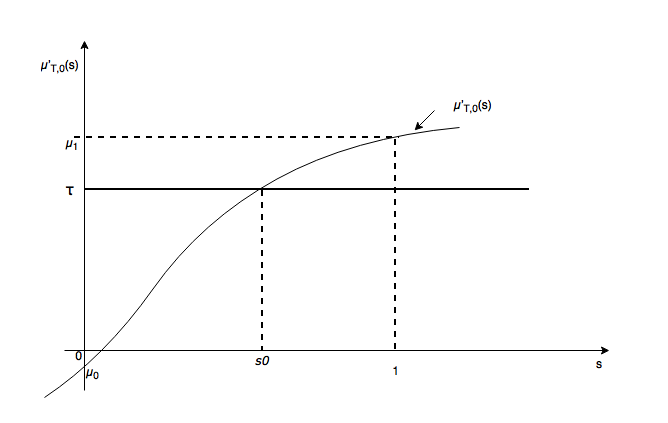
\includegraphics[scale=1]{Figures/CGF_Derivative}
\caption{Variation of  $\mu^\prime_{T,0}(s) $: the derivative of the CGF. Level $\tau$ is attained at $s = s0$}
\label{fig:Mu0dash}
\end{figure}



\newpage
\noindent  We have:


 
            \begin{equation}
            \begin{aligned}
                       \mu^\prime_{T,0}(0) &=  \frac{\partial \mu_{T,0}(s)}{\partial s}\Bigr|_{s = 0}\\
                                                          &=\frac{\partial log(E_0[e^{sT(y)}])}{\partial s}\Bigr|_{s = 0}\\
                                                          &=\frac{E_0[T(y)e^{sT(y)}]}{E_0[e^{sT(y)}]}\Bigr|_{s = 0}\\
                                                          &=E_0[T(y)]\\
                                                          &:=\mu_0\\
            \end{aligned}
            \end{equation}


Similarly,\\


              \begin{equation}
              \begin{aligned}
                   \mu^\prime_{T,0}(1) &= \frac{E_0[T(y)e^{T(y)}]}{E_0[e^T(y)]}\\
                                                     :&=\mu_1\\
              \end{aligned}
              \end{equation}

\noindent Let us analyze the important special case when $T(y)=log(L(y)) = log(\frac{P_1(y)}{P_0(y)})$.

\noindent Then,
            \begin{equation}
            \begin{aligned}
                  \label{l1}
                 \mu_0 = E_0[log(L(y))]\\
            \end{aligned}
           \end{equation}

\noindent We now introduce an inequality for Convex ( and Concave ) functions. \\ 

\noindent\textbf{\underline{Jensen's inequality:}} If X is a random variable and $f:\mathbb{R}\rightarrow \mathbb{R}$ is a convex function, then

         \begin{equation}
             \label{l2}
             f(\mathbb{E}[x])\leq \mathbb{E}[f(x)].
            \end{equation}

\noindent Also, if g is convave, then,


           \begin{equation}
            \label{l3}
         g(\mathbb{E}[x])\geq \mathbb{E}[g(x)].
            \end{equation}


\noindent Getting back to \eqref{l1}, and noting that $log$ is a concave function, the bound invoking Jensen's inequality becomes:  \\


               \begin{equation}
               \begin{aligned}
                  \label{l4}
                  \mu_0 &= E_0[log(L(y))] \leq log E_0[L(y)]\\
                             &= log(\int\limits_\Gamma \frac{P_1(y)}{P_0(y)}P_0(y)dy)\\
                             &= log(1) \\
                             &= 0
                 \end{aligned}
                 \end{equation}

\noindent We have shown that  $\mu_0 \leq 0$.\\
\noindent Similarly, we can show that $\mu_1 \geq 0$.\\

\noindent Note that $log$ is a "strictly" concave function and hence Jensen's  inequality as stated in  \ref{l3} can be replaced by a strict inequality sign.\\
                Consequently, we have  $\mu_0 < 0$ and  $\mu_1 > 0$. \\

\noindent Hence a solution to the equation \\

              \begin{center}
                  $ \mu^\prime_{T,0}(s) = \tau$\\
                 exists iff  $ \tau \in [\mu_0, \mu_1]$\\
              \end{center}


\begin{exmp}
         If $H_0: T(y) \sim \mathcal{N}(\mu,\sigma^{2}), \mu > 0 $,  then:
                  \begin{align*}
                         \mu_{T}(s)&=log(E[e^{sT(y)}]), \mu > 0\\
                                           &=s\mu + \frac{s^{2}\sigma ^{2}}{2}\\
                          \implies \mu \prime_{T}(s) &= \mu + s\sigma^{2}\\
                  \end{align*}
\end{exmp}




\noindent Notice that all these were bounds for $P_F$ and  $P_M$, derived without any mention of priors and as such; that relates to the N-P situation.We now investigate if we can say something about the bounds for Bayesian testing.

\subsection{Chernoff Bounds for Bayesian Hypothesis Testing:}

\par Let the prior be $\pi_0$ on $H_0$ and $\pi_1 = (1 - \pi_0 )$  on $ H_1 $.\\

\noindent For a rule $\delta$, the average probability of error  is:
              \begin{align}
                   &= \pi_0  E_0[\delta(Y)] + \pi_1  E_1[1- \delta(Y)]\nonumber\\
                   &= \pi_0  P_F(\delta) + \pi_1  P_M(\delta) 
                     := P_e
               \end{align}


\noindent Now, we can bound $P_e$,  $\forall s \in [0,1]$  as follows:
 

              \begin{align}
                     P_e&\leq\pi_0 e^{-s\tau + \mu_{T,0}(s) }+\pi_1 e^{(1-s)\tau +  \mu_{T,0}(s)}\nonumber \\
                           &=(\pi_0+\pi_1 e^{\tau}) e^{-s\tau + \mu_{T,0}(s) } 
              \end{align}

\noindent This is applicable whenever $\delta$ is constructed using  $T(y)\gtreqqless\tau$.
                It turns out, that we can slighly better this bound. \\

\noindent It can be shown that: \\
                \begin{align}
                    P_e\leq \max\ (\pi_0, \pi_1 e^{\tau} ) \,  e^{-s \tau + \mu_{T,0}(s)} 
                \end{align}


\noindent Now, the detector with minimum $P_e$ is simply:


                \begin{align}
                      \delta(y) = 1_{ \{ log(L(Y)) \geq log(\frac{\pi_0}{\pi_1})\}}
                \end{align}

\noindent where we have put  $T = log(L(Y))$  and  $ \tau =  log(\frac{\pi_0}{\pi_1}) $ \\

\noindent Therefore, the minimum probability of error detector achieves, $\forall s \in [0,1]$:

               \begin{align}
                        P_e&\leq\pi_0 e^{-s \:  log(\frac{\pi_0}{\pi_1}) +  \mu_{T,0}(s) } \nonumber \\
                              &= \pi_0 (\frac{\pi_0}{\pi_1})^{-s}   e^{\mu_{T,0}(s)}  \nonumber \\             
                              &= \pi_0^{(1-s)} \:  \pi_1^{s} \:  e^{\mu_{T,0}(s)} 
               \end{align}  


\noindent Thus, given the priors, this is a bound that we can derive for $P_e$, corresponding to a Bayesian setting.


\subsection{Special Case: IID Observations}

Assume every observation $\underline{\mathbf{Y}}$ is an n-dimensional vector. Our setting is:
         \begin{align*}
              \Gamma &= \mathbb{R}^n\\\\
              \mathcal{H}_0&:   \underline{\mathbf{Y}} \sim \underbrace{\mathbbm{P}_0 \times  \mathbbm{P}_0 \times ......  \times \mathbbm{P}_0}_\text{n times} \\
             \mathcal{H}_1&:   \underline{\mathbf{Y}} \sim \underbrace{\mathbbm{P}_1 \times  \mathbbm{P}_1 \times ......  \times \mathbbm{P}_1}_\text{n times} \\
         \end{align*}

\noindent Under this setting, we ask a few questions: \\
What is the nature of the relationship between the number of samples, $n$ and the Probability of error, $P_e$? 
Intuitively, we expect that as more samples become available, the probability of error must correspondingly go down. 
As we shall see, such  is indeed the case. But we also seek the explicit form of the relation between $P_e$ and $n$ to know how fast $P_e$ decays as more and more samples become available for processing.
These questions motivate the following calculations. \\

\newpage

\noindent We have:

              \begin{equation}
              \begin{aligned}
                     \mu_{T,0}(s) &=  log\Big(E_0 \Big[e^{s \: log(L(\underline{Y})  ) } \Big] \Big)  \\
                                           &=  log\Big(E_0 \Big[e^{s \: log \prod_{k=1}^{n} \big[\frac{P_1(y_k)}{P_0(y_k)}\big]  } \Big] \Big)  \\
                                           &=  log\Big( E_0 \Big[ \prod_{k=1}^{n}  e^{s \:  log \big[ \frac{P_1(y_k)}{P_0(y_k)}\big] } \Big] \Big)   \\
                                           &= \sum_{k=1}^{n} log \Big( E_0 \Big[   e^{s \: log \big[ \frac{P_1(y_k)}{P_0(y_k)}   \big]  }    \Big] \Big)  \\
                                           &= n \: log \Big( E_0 \Big[  e^{s \: log \big[\frac{ p_1(y_1)}{ p_0(y_1)} \big]}  \Big] \Big)  \\
                                           &= n \: log \Big(  E_0\Big[ \Big( \frac{ p_1(y_1)}{ p_0(y_1)} \Big)^{s}  \Big] \Big)    \\
                                           &= n \: log  \int_{y \in \Gamma} p_1^{s}(y) \: p_0^{(1-s)}(y) \: dy\\\\
              \end{aligned}
              \end{equation}

\noindent  Notice that this is linear in $n$. Define: \\
                 \begin{align}
                       log  \int_{y \in \Gamma} p_1^{s}(y) \: p_0^{(1-s)}(y) \: dy := -c(s), s \in [0,1] 
                  \end{align}

\noindent    Consider a function, $h(x) = x^{s}, s \in [0,1] $. Then $h(x)$ is  a concave function in $x$. (For example, when $ s = 1/2 $, $h(x)$ becomes the square root function, whose graph is obviously concave.)\\\\

             
\noindent  It follows that if we consider the function: $  E_0 \Big[ log  \Big( \Big( \frac{ p_1(y_1)}{ p_0(y_1)} \Big)^{s}  \Big) \Big] $, we have - by invoking Jensen's inequality: \\

              \begin{align}
                      E_0 \Big[ log  \Big( \Big( \frac{ p_1(y_1)}{ p_0(y_1)} \Big)^{s}  \Big) \Big]  &\leq   log \Big(  E_0\Big[ \Big( \frac{ p_1(y_1)}{ p_0(y_1)} \Big)^{s}  \Big] \Big) \nonumber \\
                                                                                                                                              &= 0 \:\: \text {( Paralleling the argument in \ref{l4} )  } \nonumber \\
                                                                                                                                \implies c(s) &\geq 0 \\
                     \therefore P_e &\leq \pi_0^{(1-s)} \: \pi_1^{(s)} \: e^{-n \: c(s)}, \forall s \in [0,1]
              \end{align}


\noindent \textbf{\underline{Note:-}}


\begin{enumerate}
  \item The minimum $ P_e $ decays to 0 \underline{exponentially fast}, in $n$ (no: of samples) in the IID detection problem.
  \item The best possible exponent is given by :  \Big[$\max\limits_{s \in [0,1]} c(s)$ \Big].\\
\noindent This quantity is called the \textbf{``Chernoff Information''}, denoted: $c_{max}  = \max\limits_{s \in [0,1]} c(s)$. \\
\noindent In fact,   $c_{max}  = D\Big( P \parallel P_0   \Big) $, where the R.H.S denotes the Kullback--Leibler (KL) divergence between the 2 distributions. In particular,   $c_{max}  = D\Big( P \parallel P_0   \Big)  =   D\Big( P \parallel P_1   \Big)$. \\
\end{enumerate}



\subsection{Stein's Lemma: (N--P Case)} 

\begin{exmp}
[Chernoff Bounds for the quadratic energy detector] 
 
           \begin{align*}
                  H_0 : \underline{Y}  &=\underline{N}, \; \; \; \; \; \; \; \: \underline{N} \sim \mathcal{N}( \underline{0}, \sigma^{2}\mathbb{I})  \\
                  H_1 : \underline{Y}  &=\underline{S} + \underline{N}, \; \: \underline{S} \sim \mathcal{N}( \underline{0}, \varSigma_{s}) \\ 
           \end{align*}

\noindent Recall the transformation, by virtue of SVD:

          \begin{align}
                  \varSigma_{s} =  \sum_{k=1}^{n} \lambda_k \:\underline{v_k} \:\underline{v}^\intercal 
          \end{align}

\noindent  where $\{ \underline{v_k}\}$  are orthonormal.  The quadratic energy detector is: 

            \begin{align}
                            \underline{y}^\intercal Q\underline{y}&\gtreqqless \tau \\
                            \text{where, \:} Q &=  \sigma^{-2} \:\varSigma_{s} \: (\sigma^{2}\mathbb{I}+ \varSigma_{s} )^{-1} \nonumber \\
                                                           &= \sum_{k} \frac{\lambda_k}{\sigma^{2} (\sigma^{2} + \lambda_k )} \: \underline{v_k} \; \underline{v_k}^\intercal \\
                            \text{Thus, \:} \underline{y}^\intercal Q\underline{y} &= \sum_{k=1}^{n} y_k^{2} \\
                            \text{ where\:} y_k :&= \underline{y}^\intercal \underline{v_k} \: \sqrt{ \frac{\lambda_k}{\sigma^{2} (\sigma^{2} + \lambda_k )}} \\
                             \text{under} H_j, j &\in \{0,1\}.  \nonumber
            \end{align}


\noindent Here, $\left\{y_k\right\}^{n}_{k=1}$  are independent gaussian random variables with mean 0 and variance :   $\left\{\sigma_{j,k}^{2}\right\}^{n}_{k=1}$. \\

           \begin{align}
                 \therefore \: L( \underline{y}) &=  \frac{ p_1(\underline{y})}{ p_0(\underline{y})} \nonumber \\
                                          &=   \frac{  p_1(\left\{y_k\right\}^{n}_{k=1})  }  { p_0(\left\{y_k\right\}^{n}_{k=1})  } \nonumber \\
                                          &=  \prod_{k=1}^{n} \Bigg(       \frac{  \Big(\frac{1}{\sigma_{1,k} \: \sqrt{2\pi}}\Big) e^{   \frac{-y_k^{2}}{2 \: \sigma_{1,k}^{2} }   }  } {  \Big(\frac{1}{\sigma_{0,k}\: \sqrt{2\pi}}\Big) e^{   \frac{-y_k^{2}}{2 \: \sigma_{0,k}^{2}}   }   } \Bigg) \nonumber \\
                                          &=   \prod_{k=1}^{n}  \Big( \frac{\sigma_{0,k}}{\sigma_{1,k}} \Big) \: e^{  \frac{y_k^{2}}{2}  }   \\
                       \text{Put} \: T &= log L \nonumber \\
                       \text{We have:} \: \mu_{T,0}(s) &= log \: E_0[e^{sT}] \nonumber  \\
                                                                            &= log \: E_0\Big[  \prod_{k=1}^{n}   \Big(\frac{\sigma_{0,k}}{\sigma_{1,k}} \Big)^{s} \: e^{\frac{s\:y_k^{2}}{2}  }   \Big]\\
                      \text{We see that:} \: y_k^{2} &\sim Gamma\Big (\frac{1}{2}, \frac{1}{2 \: \sigma_{0,k}^2} \Big ) \text{and,}
           \end{align}



             \begin{equation}
                     E_0[e^{\frac{s\:y_k^{2}}{2}}] = 
                \begin{cases}
                         (1 - s \: \sigma_{0,k}^2)^{-1/2}&,  s< \frac{1}{\sigma_{0,k}^2}\\
                         \infty&,  s\geq \frac{1}{\sigma_{0,k}^2}
               \end{cases}
            \end{equation}


\noindent  For the Bayesian problem, the min $P_e$ satisfies:
                     \begin{align}
                         P_e \leq \pi_0^{(1-s)} \: \pi_1^{(s)} \: e^{ \mu_{T,0}(s)} 
                     \end{align}
                         
\noindent After some manipulations, we get:
                    \begin{align}
                                 = \pi_0^{(1-s)} \: \pi_1^{(s)} \prod_{k=1}^{n} \Bigg(  \frac{\sigma^{2s} (\sigma^{2} + \lambda_k)^{\frac{1}{2} - s}}{(\sigma^{2} + (1-s)\lambda_k)^{\frac{1}{2}}}    \Bigg)
                     \end{align}

\noindent Differentiating w.r.t $s$ and setting to 0, for $ s \in [0,1] $, we get:

                     \begin{align}
                          \sum_{k=1}^{n} \Big( \frac{\lambda_k}{2(\sigma^{2} + (1-s)\lambda_k)}   \Big) =   \sum_{k=1}^{n} log\big( 1 + \frac{\lambda_k}{\sigma^{2}} \big) + log(\frac{\pi_1}{\pi_0})
                     \end{align}

\end{exmp}





	
\end{document}